\documentclass[a4paper,12pt,floatssmall]{scrartcl}

% Page geometry's formatting
\usepackage[left=2.5cm,right=2.5cm,top=2.5cm,bottom=2.5cm]{geometry}
\usepackage{indentfirst}
\usepackage{placeins}
\usepackage{float}
% Language-specific settings
\usepackage[T1]{fontenc}
\usepackage[utf8]{inputenc}
\usepackage[polish]{babel}
\usepackage{polski}
% Elements' embedding
\usepackage{listings}
\usepackage{graphicx}
\usepackage[bf]{caption}
\usepackage{subcaption}
\usepackage{hyperref}
% Text-formatting
\usepackage[autostyle]{csquotes}
\usepackage{caption}
\usepackage{moresize}
\usepackage{amsmath}
% Miscellaneous
\usepackage[backend=biber,style=ieee]{biblatex}
\usepackage[enable]{easy-todo}
\usepackage{lipsum}
\usepackage{setspace}


% ================================================================================================================================== %
% --------------------------------------------------------- Configuration ---------------------------------------------------------- %
% ================================================================================================================================== %

% Unordered list
\renewcommand{\labelitemi}{\textbullet}

% Bibliography file
\addbibresource{bibliography.bib}

% ================================================================================================================================== %
% ------------------------------------------------------- Macrodefinitions --------------------------------------------------------- %
% ================================================================================================================================== %

% Redefininiton of the title page
\renewcommand{\maketitle}{
\begin{titlepage}
    \vfill
    \begin{center}
        \begin{figure}
            \centering
            
\includegraphics[scale=0.9]{img/header.png}
            \vspace{0.5cm}
        \end{figure}
    \end{center}
    \vspace{2cm}
    \begin{center}
        {\HUGE {\textbf{Programowanie kładów FPGA}}}\\
        \vspace {0.4cm}
        {\Large {(projekt)}}
    \end{center}
    \vspace{4cm}
    \begin{center}
        {\setstretch{1.5}\textbf{\LARGE Implementacja algorytmów cyfrowego przetwarzania sygnałów audio na bazie układu FPGA z interfejsem UART}}
        \vspace{3cm}
    \end{center}
    \vfill
    \begin{center}
        {\textbf{\normalsize Pierczyk Krzysztof}}
    \end{center}
    \vfill
    \begin{center}
        \large{Warszawa, \today \par}
    \end{center}
\end{titlepage}
}

% Definition of `part` module
\renewcommand\partheadstartvskip{\clearpage\null\vfil}
\renewcommand\partheadmidvskip{\par\nobreak\vskip 20pt\thispagestyle{empty}}
\renewcommand\partheadendvskip{\vfil\clearpage}
\renewcommand\raggedpart{\centering}

% ================================================================================================================================== %
% ------------------------------------------------------------- Text --------------------------------------------------------------- %
% ================================================================================================================================== %

\begin{document}
    
% Title
\maketitle

% Table of content
\tableofcontents

% Chapter I - Theoretical analysis
\part{Analiza teoretyczna}
\section{Wstęp}

Celem projektu jest opracowanie i~zaimplementowanie zestawu wybranych metod przetwarzania sygnałów audio znanych z~popularnych multiefektów gitarowych. Zadaniem tego typu rozwiązań jest modyfikowanie próbkowanego dźwięku w~czasie rzeczywistym w taki sposób, aby urozmaicić jego brzmienie np. poprzez modulację, przesunięcie fazowe lub wprowadzenie dodatkowych składowych. Przykładami takich efektów są m.in.

\begin{itemize}
    \item \textbf{echo} (opóźnienie, ang. \textit{delay}) - do sygnału dodawana jest jedna lub kilka jego kopii opóźnionych o~określoną liczbę próbek; efekt ma symulować warunki panujące w~halach widowiskowych
    \item \textbf{overdrive} - nazwa ogółu metod prowadzących do znacznego zniekształcenia sygnału bazowego; jednym z~popularnych sposobów jego implementacji jest nałożenie obustronnych ograniczeń na wyjściowe wartości przepuszczanego sygnału
    \item \textbf{flanger} - kolejny efekt wykorzystujący opóźnione próbki sygnału; w~tym przypadku wielkość opóźnienia podlega cyklicznym zmianom, co przekłada się na pulsacyjny charakter wyjściowego dźwięku
    \item \textbf{tremolo} - efekt modulujący amplitudę sygnału zgodnie z~przebiegiem pewnej funkcji okresowej (np. sinus lub fala trójkątna); jego celem jest symulowanie rodzaju artykulacji polegającego na szybkim wydobywaniu dźwięków o~tej samej częstotliwości (np. poprzez szybkie szarpanie pojedynczej struny gitarowej) 
\end{itemize}

Powyższe efekty stanowią jedynie niewielki wycinek stosowanych rozwiązań, wśród których wymienić można także szeroko pojęte metody equalizacji, czy modyfikowania częstotliwości sygnału. Minimalna wersja projektu zakłada implementację scharakteryzowanych metod przetwarzania wraz z~prostymi mechanizmami wprowadzania i~wyprowadzania danych z~urządzenia a~także dostosowywania parametrów filtrów. Jako metodę komunikacji wybrano popularny (choć może w~niec innych zastosowaniach) interfejs UART (ang. \textit{universal asynchronous receiver-transmitter}). Jego prostota umożliwi przyspieszenie procesu implementacji, a~co za tym idzie szybsze przejście do zasadniczej części projektu. Cyfrowy charakter UARTa pozwoli w~przyszłości przejść na popularny interfejs $I^{2}S$, dzięki któremu możliwe będzie proste dołączenie do urządzenia układów przetwornikowych. Testowanie urządzenia obywać się będzie z~pomocą prostej aplikacji w~języku Python, która za pośrednictwem wirtualnego portu szeregowego wysyłać będzie do urządzenia próbki dźwięku. Sygnał wychodzący z~układu FPGA będzie następnie odtwarzany za~pomocą jednej z~wielu dostepnych w~Pythonie bibliotek audio jak np. \verb|pyaudio|.

\section{Analiza interfejsu komunikacyjnego}

Interfejs UART jest dzisiaj dostępny w~niemal wszystkich obecnych na mikrokontrolowerowych oraz w~wielu układach typu SoC. Jego popularność wynika zarówno z~(jak sama nazwa wskazuje) uniwersalnego charakteru jak i~prostoty implementacji. UART to cyfrowe urządzenie peryferyjne umożliwiające szeregową komunikację asynchroniczną. W~większości implementacji parametry komunikacji takie jak szybkość, czy format danych mogą być konfigurowane poprzez zmianę wartości odpowiednich rejestrów sterujących. Nierzadko możliwe jest też ustawienie trybu komunikacji spośród \textit{simplex}, \textit{duples} lub ~\textit{half-duples}. Interfejsy tego typu, szczególnie w~zastosowaniach przemysłowych, są często sprzęgane z~konwerterami poziomów logicznych odpowiednich dla standardów RS-232 lub RS-485.

\begin{figure}
    \centering
    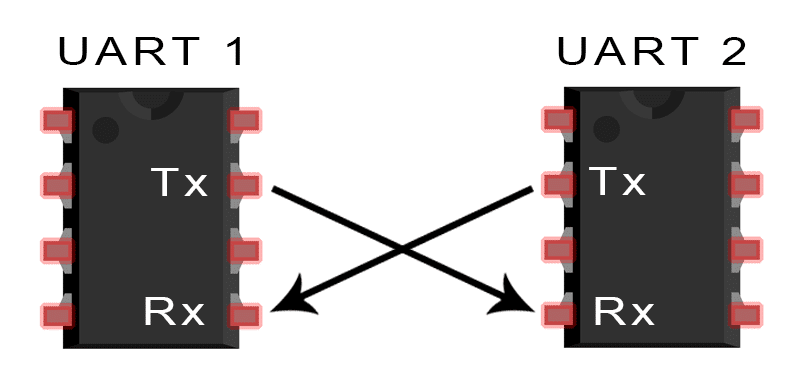
\includegraphics[scale=0.5]{img/uart.png}
    \captionsetup{format=plain,justification=centering}
    \caption{Typowa struktura komunikacji dwóch węzłów z~wykorzystaniem układu UART, źródło: \cite{uart}}
    \label{UART}
\end{figure}

Komunikacja asynchroniczna wymaga aby wszystkie węzły nadawały i~odbierały dane o~z~góry ustalonym formacie i~długości znaku (wynikającym z~szybkości transmisji). Ponadto należy wziąć pod uwagę, że zegary obecne w~poszczególnych urządzeniach mogą się z~czasem rozsynchronizowywać, a~co za tym idzie konieczny jest mechanizm ponownej synchronizacji. W~przypadku komunikacji z~wykorzystaniem modułu UART mechanizm ten wynika z~formatu przesyłanych danych. Typowa ramka składa się z~trzech elementów: \textbf{bitu startu}, \textbf{bitów danyc} oraz \textbf{bitów stopu}. Bit startu oznacza początek nowej ramki i~jest sygnalizowany stanem niskim na linii. Po nim następować może pewna liczba bitów danych - zazwyczaj $7$ lub $8$  - a~na końcu jeden lub dwa bity stopu (sygnalizowane stanem wysokim). Bit startu odpowiada za synchronizację zegarów wykorzystywanych do próbkowania stanu linii, natomiast bity stopu definiują minimalną przerwę między kolejnymi ramkami. Fakt że każdy bit startu to ponowna okazja do zsynchronizowania zegarów sprawia, że nie muszą one pracować z~dokładnie tymi samymi szybkościami. Niewielkie różnice nie powodują błędów w~odbiorze danych.

\begin{figure}
    \centering
    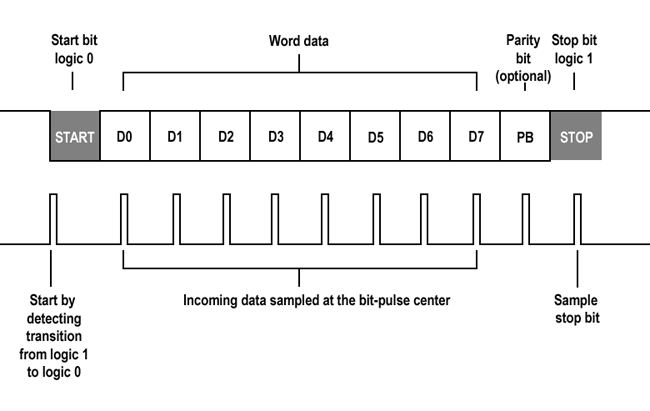
\includegraphics[scale=0.5]{img/uart_frame.png}
    \captionsetup{format=plain,justification=centering}
    \caption{Struktura ramki UART, źródło: \cite{uart_frame}}
    \label{UART}
\end{figure}

Format ramki może zostać rozszerzony o~element kontrolny w~postaci \textbf{bitu parzystości}. Jeśli występuje, przyjmuje on wartość zależną od ilości bitów w~stanie wysokim w~przesyłanych danych i~znajduje się przed bitami stopu. Możliwy jest bit parzystości (ang. \textit{even}) - ustawiony, gdy suma jest parzysta - lub nieparzystości (ang. \textit{odd}) - ustawiany, gdy suma jest nieparzysta. Dodatkowy element pozwala wykrywać ewentualne błędy transmisji. Format ramki często oznacza się w~postaci trzyznakowego identyfikatora postaci $DPS$, gdzie $D$ oznacza ilość bitów danych, $P$ - typ bitu kontrolnego ($E$ - bit parzystości, $O$ - bit nieparzystości, $N$ - brak bitu kontrolnego) a~$S$ ilość bitów stopu. Typowowymi prędkościami transmisji przez UART są:

\begin{itemize}
    \item 9600 bit/s
    \item 19200 bit/s
    \item 38400 bit/s
    \item ...
\end{itemize}

Jest to pewna zaszłość historyczna wynikająca z~częstotliwości standardowych oscylatorów dostępnych na rynku. Moduły współcześnie implementowane w~układach scalonych wzbogacone są często o~dodatkowe wyprowadzenia zegarowe umożliwiające komunikację synchroniczną. Tego typu urządzenia określane są zazwyczaj mianem USART (ang. \textit{universal synchronous asynchronous receiver-transmitter}).

% ================================================================================================================================== %
% ------------------------------------------------------------ Effects ------------------------------------------------------------- %
% ================================================================================================================================== %

\section{Efekty dźwiękowe}

Pierwszą decyzją projektową dotyczącą efektów było stworzenie jednolitego interfejsu implementaowanych bloków przetwarzających. Ma to umożliwić arbitralne połączenie ich w~potok oraz dodanie w~przyszłości nowych efektów bez wprowadzania znacznych zmian w~projekcie. Wykorzystano w~tym celu strukturę zaczerpniętą z~\cite{fpga_pedal}, która została przedstawiona na Rys.\ref{effects-pipe}.

\vspace{0.5cm}
\begin{figure}[ht]
    \centering
    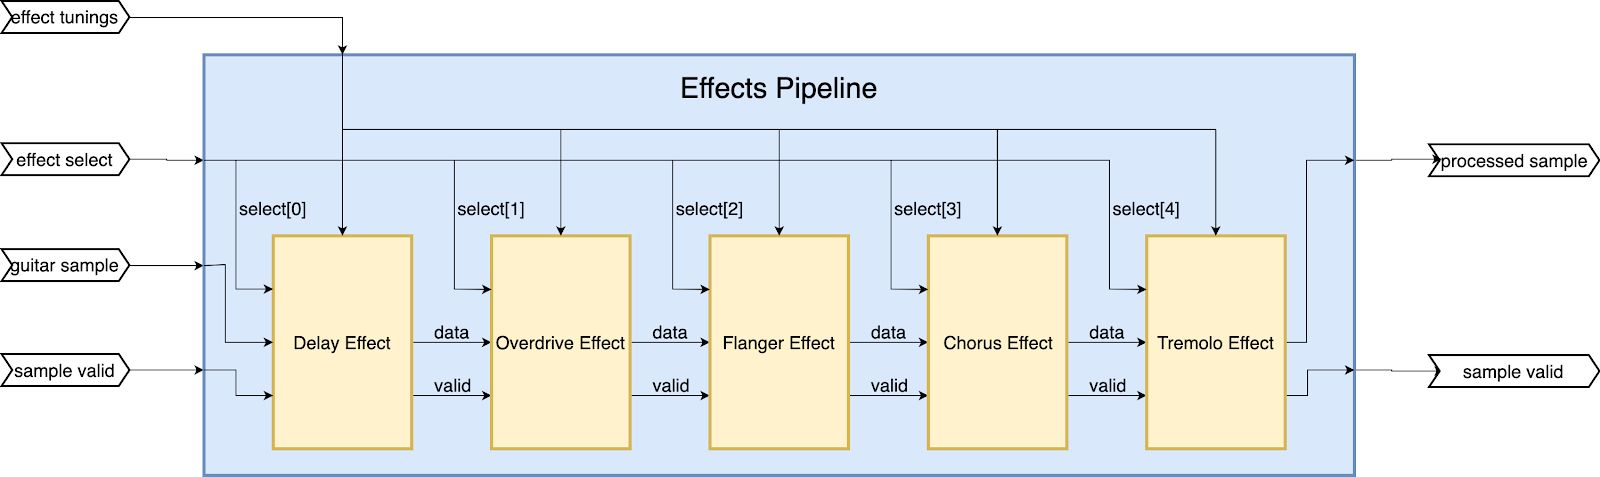
\includegraphics[scale=0.25]{img/pipe.jpg}
    \captionsetup{format=plain,justification=centering}
    \caption{Planowana struktura potoku efektów, źródło: \cite{fpga_pedal}}
    \label{effects-pipe}
\end{figure}
\vspace{0.5cm}

Każdy blok posiada trzy standardowe wejścia oraz dwa standardowe wyjścia. Projekt zakłada wykorzystanie 16-bitowych próbek dźwięku, co determinuje szerokość szyn danych. Wejścia \verb|valid| aktywowane są zboczem narastajacym i~oznaczają pojawienie się nowej próbki na wejściu bloku. Po przetworzeniu próbki moduł ma obowiązek wystawienia danych na linię wyjściową oraz wygenerowanie zbocza narastającego na wyjściu \verb|valid|, które podłączone jest do odpowiadającego wejścia następnego modułu. Każdy z~bloków posiada także jednobitowe wejście \verb|enable|. Stan niski na tej linii oznacza, że blok powinien przekazywać na swoje wyjście próbkę wejściową bez jej modyfikowania. Każdy blok może dodatkowo implementować arbitralne wejścia konfiguracyjne specyficzne dla działania danego algorytmu. W~przypadku blok \textit{overdrive} może być to na przykład 8-bitowa wartość wzmocnienia sygnału i~16-bitowe wartości górnego i~dolnego nasycenia (szczegóły opisano w~dalszej części dokumentu).

Tak zaprojektowana struktura pozwala w~łatwy sposób modyfikować obecne w~systemie efekty oraz nie nakłada ścisłych ograniczeń na interfejs użytkownika wykorzystywany do ich kontrolowania. Również sposób dostarczania i~odbierania danych z~potoku nie jest dzięki temu ograniczony do konkretnego interfejsu komunikacyjnego.

% ----------------------------------------------------------- Overdive ------------------------------------------------------------- %

\subsection{Overdrive}

Jak nakreślono we wstępie efekt przesterowania (ang. \textit{overdive}) określa zespół metod prowadzących do znacznego zniekształcenia sygnału bazowego poprzez dodanie do niego dodatkowych składowych harmonicznych. Częstym sposobem implementacji takiego efektu jest obustronne przycinanie sygnału wejściowego. W~niniejszym projekcie zastosowana zostanie struktura przedstawiona na Rys. {effects-overdrive}.

\vspace{0.5cm}
\begin{figure}[ht]
    \centering
    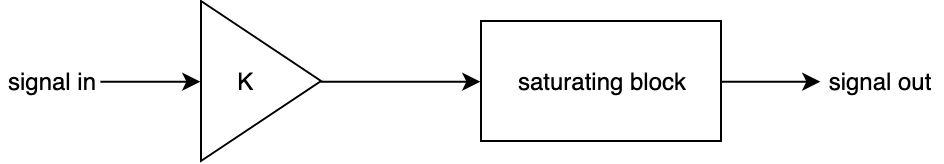
\includegraphics[scale=0.4]{img/overdrive.jpg}
    \captionsetup{format=plain,justification=centering}
    \caption{Schemat bloku \textit{overdrive}, źródło: \cite{fpga_pedal}}
    \label{effects-overdrive}
\end{figure}
\vspace{0.5cm}

Pierwszym etapem przetwarzania jest tutaj wzmocnienie sygnały wejściowego o~wartość kontrolowaną przez rejestr wejsciowy bloku. Zakres potencjalnego wzmocnienia zostanie ustalony na etapie testowania układu. Będzie ono realizowane poprzez 16-bitowe mnożenie z~nasyceniem. Wzmocniony sygnał zostaje następnie przepuszczony przez blok nasycenia. Jeżeli jego wartość mieści się pomiędzy skonfigurowanymi poziomami zostaje on podany na wyjście bez dalszych modyfikacji. W~przeciwnym wypadku na wyjściu pojawia się odpowiednia wartość nasycenia. Funkcjonalność ta może zostać zaimplementowana przy użycia dwóch 16-bitowych komparatorów oraz multipleksera.

% ------------------------------------------------------------ Delay --------------------------------------------------------------- %

\subsection{Delay}

Efekt pogłosu uzyskiwany jest poprzez sumowanie przychodzących próbek z~próbkami opóźnionymi o~określoną liczbę cykli. Realizacja takiego bloku może bazować na filtrze typu FIR (ang. \textit{Finite Impulse Response}) lub IIR (ang. \textit{Infinite Impulse Response}). W~przypadku pierwszego z~nich przeszłe próbki są opóźnionymi wersjami \textbf{sygnału wejściowego}. Liczba próbek sumowanych może być stała lub parametryzowana. Drugi sposób implementacji przewiduje sumowanie pórbki wejściowej jedynie z~jedną wersją opóźnioną sygnału. Wersja ta jest jednak pobierana z~\textbf{wyjścia układu}, co oznacza, że jest ona zależna od wszystkich poprzednich próbek sygnału. Właśnie to rozwiązanie zostanie zastosowane w~niniejszym projekcie. Jego struktura została przedstawiona na Rys.\ref{effects-delay}. W~celu uzyskania stabilnego układu konieczne jest wprowadzenia tłumienia sygnału opóźnionego. Kierując się informacjami zawartymi w~\cite{fpga_pedal} wartości tego tłumienia przyjęto w~zakresie od $0$ do $0.5$. W~celu otrzymania takiego zakresu wyjście z~bloku mnożącego będzie przepusówane o~8~bitów w~prawo (tj. dzielone przez 256).

\vspace{0.5cm}
\begin{figure}[ht]
    \centering
    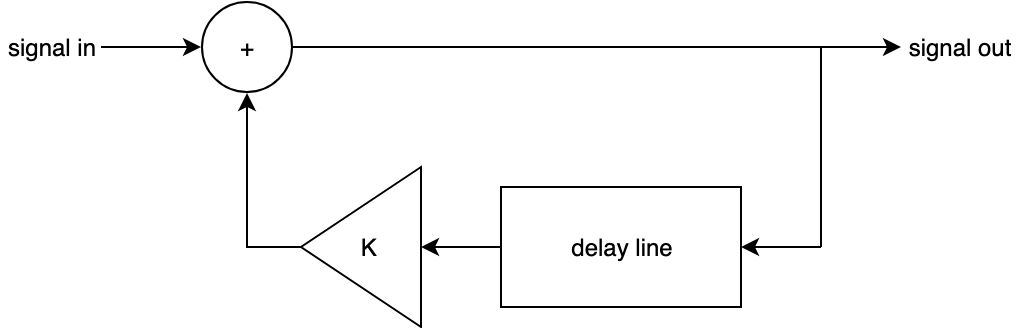
\includegraphics[scale=0.4]{img/delay.jpg}
    \captionsetup{format=plain,justification=centering}
    \caption{Schemat bloku \textit{delay}, źródło: \cite{fpga_pedal}}
    \label{effects-delay}
\end{figure}
\vspace{0.5cm}

Od strony technicznej implementacyja takiego bloku wymaga układu mnożącego, kolejki typu FIFO oraz multipleksera. Siła tłumienia echa ustalana jest poprzez wartość jednego z~wejść do układu mnożącego. Głębokość echa definiuje z~kolei indeks rejestru w~kolejce, którego wartość wystawiana jest na wyjście modułu opóźniającego. Oba parametry efektu regulowane będą przez rejestry wejściowe bloku. Maksymalna głębokość kolejki zostanie ustalona na etapie testowania.

% ----------------------------------------------------------- Flanger -------------------------------------------------------------- %

\subsection{Flanger}

\textit{Flagner} jest efektem, którego brzmienie trudno opisać, jednak zasada jego działania jest stosunkowo prosta. Efekt ten powstaje poprzez nałożenie na sygnał filtru grzebieniowego, którego charakterystyka amplitudowa wykonuje sinusoidalne oscylacje w~okół ustalonego punktu. W~prakyce układ taki realizuje się poprzez sumowanie sygnału z~jego opóźnionymi (nieprzetworzonymi) wersjami. Wartość tego opóźnienia jest jednak okresowo zmienna. Struktura takiego rozwiązania przedstawiona została na Rys.\ref{effects-flanger}. Aby kontrolować siłę efektu do ukłądu wprowadzone zostaną dodatkowe bloki tłumienia. Ich wartość zawierać się będzie w~przedziale od $0$~do $1$, natomiast ich suma będzie stale równa $1$. Podobnie jak w~przypadku pogłosu wykorzystywana głębokość kolejki FIFO (a~tym samym efektywna amplituda oscylacji wartości opóźnienia) będzie ustalana porpzez zewnętrzny parametr.

\vspace{0.5cm}
\begin{figure}[ht]
    \centering
    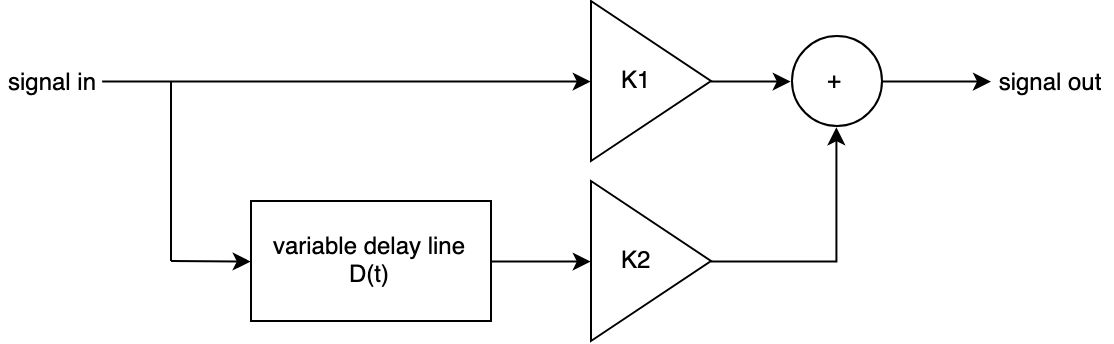
\includegraphics[scale=0.4]{img/flanger.jpg}
    \captionsetup{format=plain,justification=centering}
    \caption{Schemat bloku \textit{flanger}, źródło: \cite{fpga_pedal}}
    \label{effects-flanger}
\end{figure}
\vspace{0.5cm}

Implementacja efektu będzie wykorzystywac bloki stworzone podczas realizacji poprzedniego efektu takie jak układy mnożące oraz kolejka FIFO. Dodatkowym elementem będzie tutaj generator funkcji sinus o~zmiennej częstotliwości. Czestotliwość ta będzie również ustalana poprzez zewnętrzny parametr.

% ----------------------------------------------------------- Tremolo -------------------------------------------------------------- %

\subsection{Tremolo}

Efekt tremolo uzyskuje się poprez modulację amplitudy sygnału wejściowego. Jest to realizowane poprzez mnożenie sygnału z~pewną funkcją okresową jak np. sinus lub fala trójkątna. W~projekcie zaimplementowane zostaną oba rodzaje modulacji. Po wykonaniu testów wybrany zostanie ten, który będzie pozwalał uzyskać ciekawsze brzmienie. Schemat blokowy rozwiązania został przedstawiony na Rys.\ref{effects-tremolo}. Podobnie jak w~przypadku pogłosu wykorzystane zostanie tu 8-bitowe przesówanie wyniku mnożenia celem uzyskania efektywnej amplitudy fali modulującej w~zakresie od $0$ do $1$ (przy załżeniu, że wyjście z~generatora fali ma wartość 8-bitową).

\vspace{0.5cm}
\begin{figure}[ht]
    \centering
    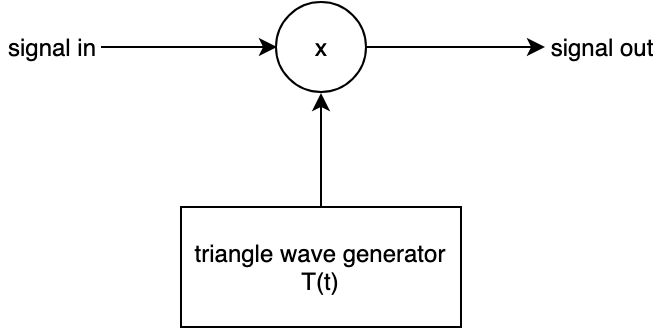
\includegraphics[scale=0.4]{img/tremolo.jpg}
    \captionsetup{format=plain,justification=centering}
    \caption{Schemat bloku \textit{tremolo}, źródło: \cite{fpga_pedal}}
    \label{effects-tremolo}
\end{figure}
\vspace{0.5cm}
% ================================================================================================================================== %
% ---------------------------------------------------------- Interface ------------------------------------------------------------- %
% ================================================================================================================================== %

\section{Interfejs użytkownika}

Ostatnim elementem projektu jest zaimplementowanie wygodnego interfejsu użytkownika. Powinien on umożliwiać niezależną aktywację każdego z~efektów oraz pozwalać na regulowanie ich parametrów. Układ FPGA udostępniać będzie cztery wejścia cyfrowe (przyciski). Zostaną one podłączone (za pośrednictwem przerzutników) do wejść \verb|enable| poszczególnych bloków przetwarzających. Aktywacja efektu możliwa będzie dzięki zmianie stanu przełącznika. Kontrola parametrów bloków przetwarzana zostanie zrealizowana za pomocą potencjometrów. Ich interfejs może zostać stworzony na dwa sposoby. Ostateczny wybór zostanie podjęty po głęszbym przeanalizowaniu zagadnienia. 

Pierwszym pomysłem jest wykorzystanie modułu XADC od Xilinx. Pozwoliłoby to na podłączenie wszystkich potencjometrów do układu FPGA z~wykorzystaniem multipleksera analogowego (np. CD74HC4067), którego wejście przełączane byłoby z~pewną częstotliwością przez układ sterujący. Wymagałoby to jednak wykorzystanie gotowego bloku IP oraz stworzenia odpowiedniego interfejsu od strony aplikacji.

Drugim pomysłem jest wdrożenie dodatkowego modułu UART, który komunikowałby się z~zewnętrznym mikrokontrolerem realizującym pomiar napięć na potencjometrach poprzez wbudowane kanały przetwornika A/C. W~takim przypadku układ FPGA odpytywałby podrzędny względem niego mikrokontroler w~sposób cykliczny, pozyskując cyfrowe wartości orientacji potencjometrów. Niezależnie od wyboru metody cyfrowe wartości pomiarów zostaną podłączone poprzez przerzutniki do wejśc konfiguracyjnych odpowiendich bloków przetwarzających sygnały.

% ================================================================================================================================== %
% --------------------------------------------------------- Simulations ------------------------------------------------------------ %
% ================================================================================================================================== %

\section{Planowane symulacje}

Planowane symulacje można podzielić na dwie zasadnicze kategorie. Pierwsza z~nich obejmuje proste testy jednostkowe \textbf{w~skali mikro}. Mowa tu o~modułach takich jak generator taktowania dla UARTa, układ mnożący, czy generator fali trójkątnej wykorzystywany w~algorytmach przetwarzania sygnału. Każdemu z~tych elementów powinien odpowiadać prosty podprojekt typu \textit{testbench}, który weryfikuje poprawność jego działania. Chociaż tworzenie tak drobnych elementów symulacyjnych może być do pewnego stopnia uciążliwe przy większej ilości testowanych elementów, to jednak doświadczenie pochodzące z~programowania pokazuje, że pozwala to zapobiec eskalacji wpływu drobnych błędów na działanie systemu jako całości.

Drugą kategorią symulacji będą testy systemowe sprawdzające \textbf{makroskopowe} działanie poszczególnych bloków funkcjonalnych. Tutaj również każdy z~modułów powinien otrzymać dedykowany projekt testowy. W~tym przypadku poza poprawnością działania podsystemów zostanie również zweryfikowana ich wydajność. Oszacowanie czasów przetwarzania danych przez dany blok funkcjonalny oraz jego złożoność przestrzenna (wymagana liczba zasobów układu FPGA) pozwolą z~jednej strony określić warunki krańcowe ich funkcjonowania, a~z~drugiej oszczować potencjalne możliwości rozwoju systemu np. o~dodatkowe efekty.

% ================================================================================================================================== %
% ------------------------------------------------------------ Tests --------------------------------------------------------------- %
% ================================================================================================================================== %

\section{Planowane testy}

Pierwszym testem poprawności działaniu układu będzie oczywiście empiryczna ocena dźwięku uzyskanego za pomocą poszczególnych efektów. Pozwoli ona nie tylko wykryć potencjalne błędy w~algorytmach przetwarzania (objawiające się np. wprowadzaniem nadmiernego szumu), ale także dostosować stałe parametry układu takie jak długości zastosowanych kolejek FIFO. 

Drugi krok weryfikacji rozwiązania zostanie zrealizowany dzięki zastosowanemu interfejsowi danych w~postaci aplikacji języka Python. Fakt, że posiadać będzie ona dostęp zarówno do surowych jak~i przetworzonych danych pozwoli w~łatwy sposób wyrysować wykresy przedstawiające przebiegi sygnałów i~np. ich transformaty. Możliwe będzie dzięki temu dokładne przyjrzenie się efektom działania poszczególnych filtrów celem wykrycia źródeł potencjalnych problemów. 

% ================================================================================================================================== %
% ----------------------------------------------------------- Platform ------------------------------------------------------------- %
% ================================================================================================================================== %

\section{Wybór platformy}

Ostateczny wybór platformy zostanie dokonany po stworzeniu fundamentów projektu pozwalających oszacować wymagania urządzenia dotyczące zasobów układu FPGA. Na ten moment potencjalny wybór został zawężony do trzech zestawów ewaluacyjnych. Pierwszy z~nich to \textbf{Digilent Cmod A7} wyposażony w~moduł XC7A35T-1CPG236C z~rodziny Artix-7. Niewielkie rozmiary oraz cena nieprzekraczająca 400zł są największymi zaletami tego wariantu. Został on wyposażony w~8-bitową pamięć SRAM o pojemności 512KB oraz pamięć szeregową Quad-SPI wielkości 4MB. Druga z~rozważanych platform to \textbf{Digilent Arty S7}. Jest to układ bardziej rozbudowany od poprzedniego. Posiada on na pokładzie moduł XC7S50-1CSGA324C (Spartan-7) zawierający ponad $50\%$ więcej bloków logicznych. Sama płytka oferuje ponadto kilka diod LED, przełączników mono- i~bistabilnych oraz cztery złącza Pmod. Cena tej platformy jest o~około $18\%$ wyższa, co oznacza wysoki stosunek zasobów do ceny, jednak liczyć się trzeba ze znacznie większymi wymiarami płytki.

Trzecim wariantem jest z~kolei zestaw \textbf{Digilent Cora Z7}. Jest to układ najuboższy w~bloki logiczne a~przy tym wyceniany na podobnym poziomie co Arty S7. Posiada on jednak układ XC7Z007S-1CLG400C z~rodziny Zynq co oznacza, że poza modułem FPGA zawiera on również jednordzeniowy procesor w~architekturze ARM Cortex-A9. Zestaw ten brany jest pod uwagę jedynie ze względu na prywatną sympatię autora do mikrokontrolerów bazujących na architekturze Cortex-M i~wynikającej z~niej chęci zapoznania się z~architekturą aplikacyjną rodziny ARM. Wariant ten zostanie wybrany wówacz, jeżeli zasoby zawartego w~nim modułu FPGA okażą się wystarczające do zaimplementowania tworzonego rozwiązania.

% Chapter II - Implementation
\part{Implementacja}
% Plan części implementacyjnej
% 1. Struktura projektowa
% 2. Interfejs komunikacyjny
%     - moduł UART
%        - schemat blokowy z opisem parameterów
%        - automat skończony
%        - symulacje
%     - bufory odbiorczy i~nadawczy
%        - schemat blokowy z opisem parameterów
%        - automat skończony
%        - symulacje
% 3. Interfejs analogowy
%     - konfiguracja XADC
%     - wrapper XADC IP Core
%     - schemat blokowy skanera z opisem parameterów
%     - automat skończony skanera
%     - symulacje
%        - skrypt generujący przebieg sygnałów analogowych
% 4. Bloki DSP
%     - symulacje
% 5. Generatory
%     - trójkątny
%        - schemat blokowy z opisem parameterów
%     - symetryczny
%        - schemat blokowy z opisem parameterów
%     - symulacje
% 6. Efekt `overdrive'
%     - schemat blokowy z opisem parameterów
%     - automat skończony
%     - symulacje
% 7. Efekt `tremolo'
%     - schemat blokowy z opisem parameterów
%     - automat skończony
%     - konfigruacja bloku BRAM
%     - symulacje
% 8. Efekt `delay'
%     - schemat blokowy z opisem parameterów
%     - automat skończony
%     - konfigruacja bloku BRAM
%     - symulacje
% 9. Efekt `flanger'
%     - schemat blokowy z opisem parameterów
%     - automat skończony
%     - konfigruacja bloków BRAM
%     - symulacje
% 10. Potok
%     - konfiguracja
%     - symulacje
% 11. Integracja
%     - symulacje
% 12. Podsumowanie
\section{Analiza interfejsu komunikacyjnego}

Interfejs UART jest dzisiaj dostępny w~niemal wszystkich obecnych na mikrokontrolowerowych oraz w~wielu układach typu SoC. Jego popularność wynika zarówno z~(jak sama nazwa wskazuje) uniwersalnego charakteru jak i~prostoty implementacji. UART to cyfrowe urządzenie peryferyjne umożliwiające szeregową komunikację asynchroniczną. W~większości implementacji parametry komunikacji takie jak szybkość, czy format danych mogą być konfigurowane poprzez zmianę wartości odpowiednich rejestrów sterujących. Nierzadko możliwe jest też ustawienie trybu komunikacji spośród \textit{simplex}, \textit{duples} lub ~\textit{half-duples}. Interfejsy tego typu, szczególnie w~zastosowaniach przemysłowych, są często sprzęgane z~konwerterami poziomów logicznych odpowiednich dla standardów RS-232 lub RS-485.

\begin{figure}
    \centering
    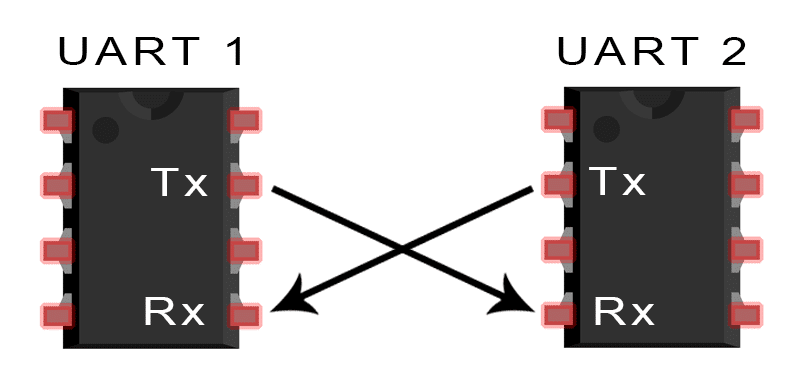
\includegraphics[scale=0.5]{img/uart.png}
    \captionsetup{format=plain,justification=centering}
    \caption{Typowa struktura komunikacji dwóch węzłów z~wykorzystaniem układu UART, źródło: \cite{uart}}
    \label{UART}
\end{figure}

Komunikacja asynchroniczna wymaga aby wszystkie węzły nadawały i~odbierały dane o~z~góry ustalonym formacie i~długości znaku (wynikającym z~szybkości transmisji). Ponadto należy wziąć pod uwagę, że zegary obecne w~poszczególnych urządzeniach mogą się z~czasem rozsynchronizowywać, a~co za tym idzie konieczny jest mechanizm ponownej synchronizacji. W~przypadku komunikacji z~wykorzystaniem modułu UART mechanizm ten wynika z~formatu przesyłanych danych. Typowa ramka składa się z~trzech elementów: \textbf{bitu startu}, \textbf{bitów danyc} oraz \textbf{bitów stopu}. Bit startu oznacza początek nowej ramki i~jest sygnalizowany stanem niskim na linii. Po nim następować może pewna liczba bitów danych - zazwyczaj $7$ lub $8$  - a~na końcu jeden lub dwa bity stopu (sygnalizowane stanem wysokim). Bit startu odpowiada za synchronizację zegarów wykorzystywanych do próbkowania stanu linii, natomiast bity stopu definiują minimalną przerwę między kolejnymi ramkami. Fakt że każdy bit startu to ponowna okazja do zsynchronizowania zegarów sprawia, że nie muszą one pracować z~dokładnie tymi samymi szybkościami. Niewielkie różnice nie powodują błędów w~odbiorze danych.

\begin{figure}
    \centering
    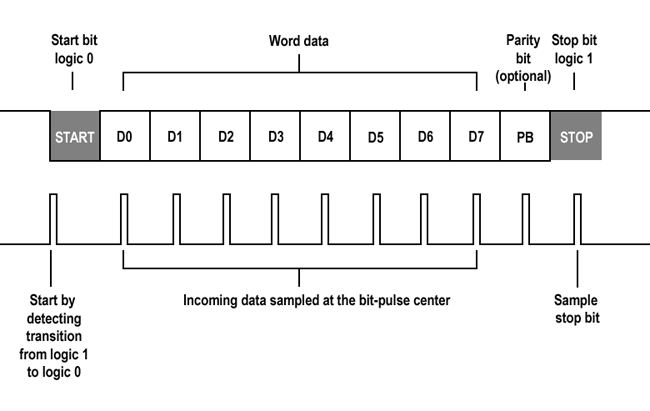
\includegraphics[scale=0.5]{img/uart_frame.png}
    \captionsetup{format=plain,justification=centering}
    \caption{Struktura ramki UART, źródło: \cite{uart_frame}}
    \label{UART}
\end{figure}

Format ramki może zostać rozszerzony o~element kontrolny w~postaci \textbf{bitu parzystości}. Jeśli występuje, przyjmuje on wartość zależną od ilości bitów w~stanie wysokim w~przesyłanych danych i~znajduje się przed bitami stopu. Możliwy jest bit parzystości (ang. \textit{even}) - ustawiony, gdy suma jest parzysta - lub nieparzystości (ang. \textit{odd}) - ustawiany, gdy suma jest nieparzysta. Dodatkowy element pozwala wykrywać ewentualne błędy transmisji. Format ramki często oznacza się w~postaci trzyznakowego identyfikatora postaci $DPS$, gdzie $D$ oznacza ilość bitów danych, $P$ - typ bitu kontrolnego ($E$ - bit parzystości, $O$ - bit nieparzystości, $N$ - brak bitu kontrolnego) a~$S$ ilość bitów stopu. Typowowymi prędkościami transmisji przez UART są:

\begin{itemize}
    \item 9600 bit/s
    \item 19200 bit/s
    \item 38400 bit/s
    \item ...
\end{itemize}

Jest to pewna zaszłość historyczna wynikająca z~częstotliwości standardowych oscylatorów dostępnych na rynku. Moduły współcześnie implementowane w~układach scalonych wzbogacone są często o~dodatkowe wyprowadzenia zegarowe umożliwiające komunikację synchroniczną. Tego typu urządzenia określane są zazwyczaj mianem USART (ang. \textit{universal synchronous asynchronous receiver-transmitter}).


% Bibliography
\clearpage
\printbibliography

\end{document}


